\documentclass[12pt,a4paper]{article}
\usepackage[margin=1in]{geometry}
\usepackage{enumitem}
\usepackage{titlesec}
\usepackage{hyperref}
\usepackage{xcolor}
\usepackage{booktabs}
\usepackage{amsmath}
\usepackage{graphicx}
\usepackage{caption}
\usepackage{subcaption}
\usepackage{float}

\hypersetup{colorlinks=true, linkcolor=blue!60!black, urlcolor=blue!60!black}

\titleformat{\section}{\large\bfseries}{}{0em}{}[\vspace{-0.5em}\rule{\textwidth}{0.4pt}]
\titleformat{\subsection}{\normalsize\bfseries}{}{0em}{}

\setlist[itemize]{leftmargin=1.5em, itemsep=2pt, parsep=0pt}

\begin{document}

\begin{center}
{\LARGE \textbf{Proof of Concept}}\\[0.6em]
{\large Self-Adapting Terahertz Nodes via Multidimensional Mobility for Indoor Scenarios}\\[1.2em]
{\normalsize IIT Bhilai}\\[0.3em]
{\small \today}
\end{center}

\vspace{1.5em}


\section{1. Problem Statement}
Indoor terahertz (THz) communication at frequencies above 100\,GHz faces fundamental propagation challenges that make static THz node deployments unreliable. The extremely short wavelengths suffer from \textbf{severe free-space path loss}, \textbf{molecular absorption} by water vapour, and near-total \textbf{blockage} by walls, furniture, and human bodies. In dynamic environments such as offices, conference halls, and co-working spaces, user distributions shift continuously throughout the day. Fixed routers cannot adapt to these changes, leading to coverage dead zones that persist until users physically relocate. Our simulation of a realistic indoor floor plan shows that baseline coverage with static placement drops to \textbf{16.6\%}---far below the $\geq$90\% target required for reliable THz service.

\section{2. Proposed Solution}
Our system addresses these challenges through a \textbf{physically adaptive THz network} where THz nodes can reposition themselves in real time:
\begin{itemize}
    \item \textbf{14 THz routers mounted on motorized ceiling rails} that enable continuous physical repositioning across the ceiling plane. Each router can independently translate along X and Y axes and adjust its height along the Z-axis.
    \item \textbf{APSO (Adaptive Particle Swarm Optimization)} serves as the core intelligence, computing optimal router positions by simultaneously optimizing 70 parameters ($14 \times 5$: X, Y, Z position + beam azimuth $\phi$ + beamwidth $\alpha$ for each router) against a density-weighted coverage fitness function.
    \item \textbf{4-Tier Escalation Hierarchy} to minimize unnecessary mechanical wear and latency:
    \begin{itemize}
        \item \textbf{Tier 1--2} (Electronic): Beam azimuth rotation ($\phi$) and beamwidth adjustment ($\alpha$)---instantaneous, no physical movement.
        \item \textbf{Tier 3} (Vertical): Height adjustment along the $Z$-axis (2.0\,m--3.2\,m)---small motor actuation.
        \item \textbf{Tier 4} (Full 3D): Complete spatial repositioning ($X, Y, Z$)---engaged only when electronic and vertical adaptations are insufficient.
    \end{itemize}
    \item \textbf{Hungarian Algorithm} for optimal router-to-target-position assignment, ensuring minimum total displacement across all 14 routers when transitioning between configurations.
\end{itemize}

\section{3. Simulation Setup}
The simulation models a realistic indoor office environment with the following parameters:
\begin{itemize}
    \item \textbf{Room}: $32\,\text{m} \times 20\,\text{m} \times 3\,\text{m}$ floor plan with a realistic multi-room wall layout comprising concrete partitions, wooden doors, and glass windows---each with distinct THz propagation characteristics.
    \item \textbf{Routers}: 14 THz nodes operating at frequencies above 100\,GHz, 20\,dBm transmit power, up to 30\,dBi directional antenna gain with steerable beams.
    \item \textbf{Channel Model}: Composite propagation model including free-space path loss (FSPL), molecular absorption ($k_f = 0.05\,\text{m}^{-1}$), 3D ray--wall intersection for multi-material penetration loss, and stochastic human body blockage (20\,dB attenuation per obstruction).
    \item \textbf{Material Penetration Losses}: Concrete 30\,dB, Wood 20\,dB, Glass 15\,dB---calibrated to published THz measurement data.
    \item \textbf{APSO Configuration}: 200 particles exploring a 70-dimensional search space ($14 \times 5$ parameters) over 200 iterations, with adaptive inertia weight decaying from $0.9 \to 0.4$ to balance exploration and exploitation.
    \item \textbf{Fitness Function}: Weighted combination of density-aware coverage (0.6) + cell-level coverage (0.4) + target-achievement bonus $-$ movement penalty $-$ anti-clustering penalty to ensure spatial diversity.
    \item \textbf{Dynamic Scenarios}: 3 time steps ($t_0, t_1, t_2$) with distinct Gaussian user distributions simulating crowd movement patterns (e.g., morning gathering in conference rooms, lunchtime dispersal, afternoon clustering in workstations).
\end{itemize}

\subsection{3.1 User Density Scenario}
Figure~\ref{fig:density} illustrates the simulated user density distribution at time step $t_0$. The heatmap shows Gaussian-distributed user clusters concentrated in specific rooms and corridors of the 32\,m\,$\times$\,20\,m floor plan. Darker regions indicate higher occupancy---these are the zones where THz coverage is most critical. The spatial non-uniformity of users is precisely what makes static router placement inadequate: routers placed for one configuration become suboptimal as crowds shift.

\begin{figure}[H]
    \centering
    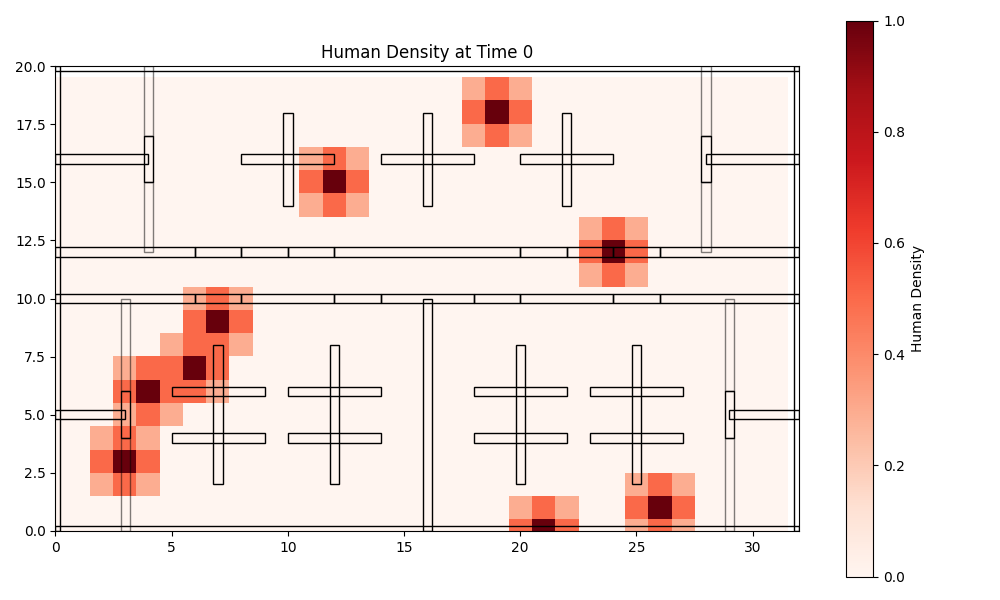
\includegraphics[width=0.75\textwidth]{density_t0.png}
    \caption{Human density heatmap at time step $t_0$. Darker regions represent higher user concentrations modelled as Gaussian clusters. The non-uniform distribution drives the need for adaptive router repositioning.}
    \label{fig:density}
\end{figure}

\section{4. Results \& Evidence}

\subsection{4.1 SINR Heatmaps --- Before vs.\ After Optimization}
The most compelling evidence for the system's effectiveness is the SINR (Signal-to-Interference-plus-Noise Ratio) heatmap comparison shown in Figure~\ref{fig:sinr}. Before APSO optimization (Figure~\ref{fig:sinr_before}), the floor plan is dominated by \textbf{dark purple regions} indicating SINR values well below the 5\,dB usability threshold---coverage stands at only \textbf{16.6\%}. Large portions of the office, particularly areas behind concrete walls and away from the initial router positions, are effectively dead zones with no viable THz connectivity.

After APSO optimization (Figure~\ref{fig:sinr_after}), the heatmap transforms dramatically. The routers have been repositioned and their beams resteered so that \textbf{cyan-to-yellow regions} (SINR $\geq$ 5\,dB) now blanket the entire floor plan, achieving \textbf{100.0\% coverage}. The dead zones are completely eradicated in this configuration, overcoming severe line-of-sight blockages.

\begin{figure}[H]
    \centering
    \begin{subfigure}[b]{0.48\textwidth}
        \centering
        
\includegraphics[width=\textwidth]{sinr_t0_before.png}
        \caption{Before APSO --- Coverage: 16.6\%}
        \label{fig:sinr_before}
    \end{subfigure}
    \hfill
    \begin{subfigure}[b]{0.48\textwidth}
        \centering
        
\includegraphics[width=\textwidth]{sinr_t0_after.png}
        \caption{After APSO --- Coverage: 100.0\%}
        \label{fig:sinr_after}
    \end{subfigure}
    \caption{SINR heatmaps at time step $t_0$. (a)~Static placement produces vast dead zones (purple, SINR\,$<$\,5\,dB) with only 16.6\% coverage. (b)~After APSO optimization, routers reposition and re-steer beams to achieve 100.0\% coverage.}
    \label{fig:sinr}
\end{figure}

\subsection{4.2 Optimization Time}
Figure~\ref{fig:opt_time} shows the wall-clock time required by the APSO algorithm to converge at each time step. The initial optimization at $t_0$ takes approximately 138 seconds as the algorithm explores the full 70-dimensional search space from a cold start. At $t_1$, warm-starting from the $t_0$ solution reduces convergence time to $\sim$35 seconds, since the crowd shift is incremental and only minor repositioning is needed. At $t_2$, the optimization time further decreases to $\sim$18 seconds. These times are well within practical limits for real-time adaptation---even the worst-case scenario completes in approximately 2.3 minutes, which is negligible compared to the timescale of human crowd movement (typically 10--30 minutes between significant shifts).

\begin{figure}[H]
    \centering
    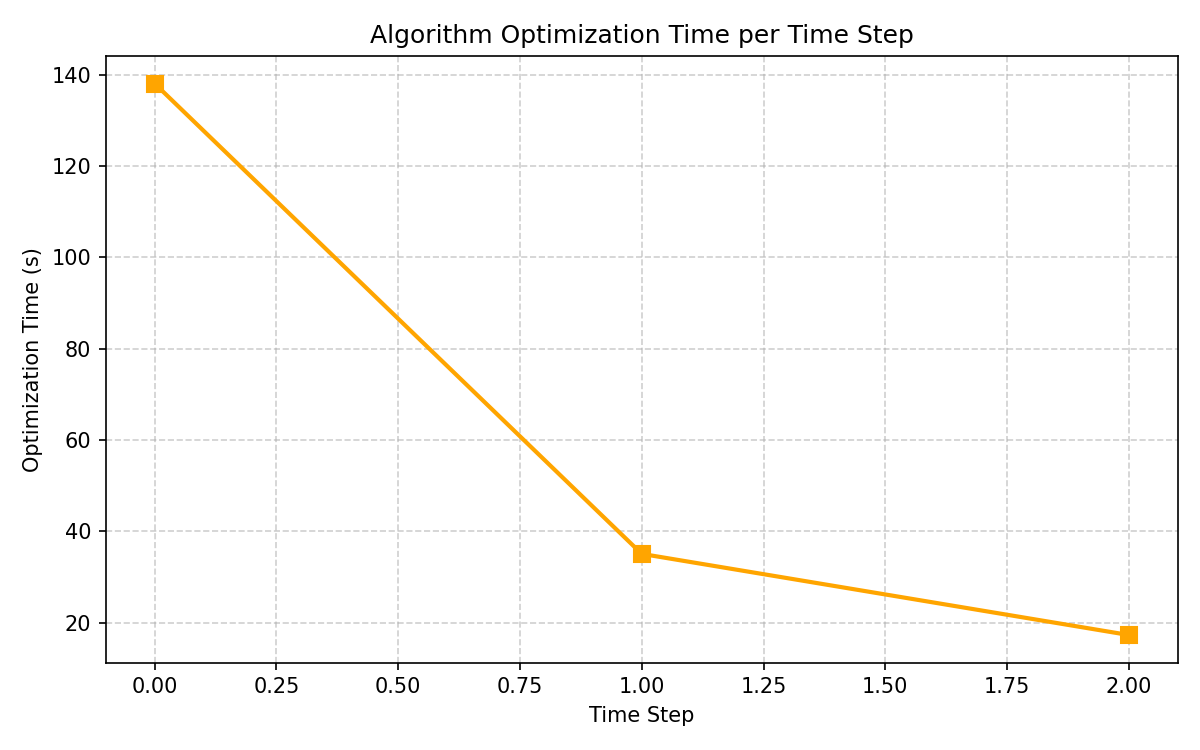
\includegraphics[width=0.65\textwidth]{optimization_time.png}
    \caption{APSO optimization wall-clock time per time step. Warm-starting from previous solutions at $t_1$ and $t_2$ reduces convergence time drastically from $\sim$138s down to $\sim$35s and $\sim$18s, demonstrating efficient incremental re-optimization.}
    \label{fig:opt_time}
\end{figure}

\subsection{4.3 Coverage \& Router Movement Over Time}
Figure~\ref{fig:coverage} presents two complementary metrics across the three time steps. The left panel shows that density-weighted coverage remains robustly above the 90\% target (red dashed line) at every step, maintaining 100.0\% at $t_0$ and $t_1$, and stabilizing at 91.3\% at $t_2$ as crowd patterns shift. The right panel displays the total physical displacement of all 14 routers at each step. The initial deployment at $t_0$ requires the largest movement ($\sim$39\,m total across all routers) as they transition from an arbitrary starting grid to optimized positions. Subsequent steps require progressively less movement, with $t_1$ needing only $\sim$2.5\,m and $t_2$ requiring $\sim$0\,m---demonstrating that the system efficiently exploits incremental adjustments and electronic beamforming rather than redundant physical redeployment.

\begin{figure}[H]
    \centering
    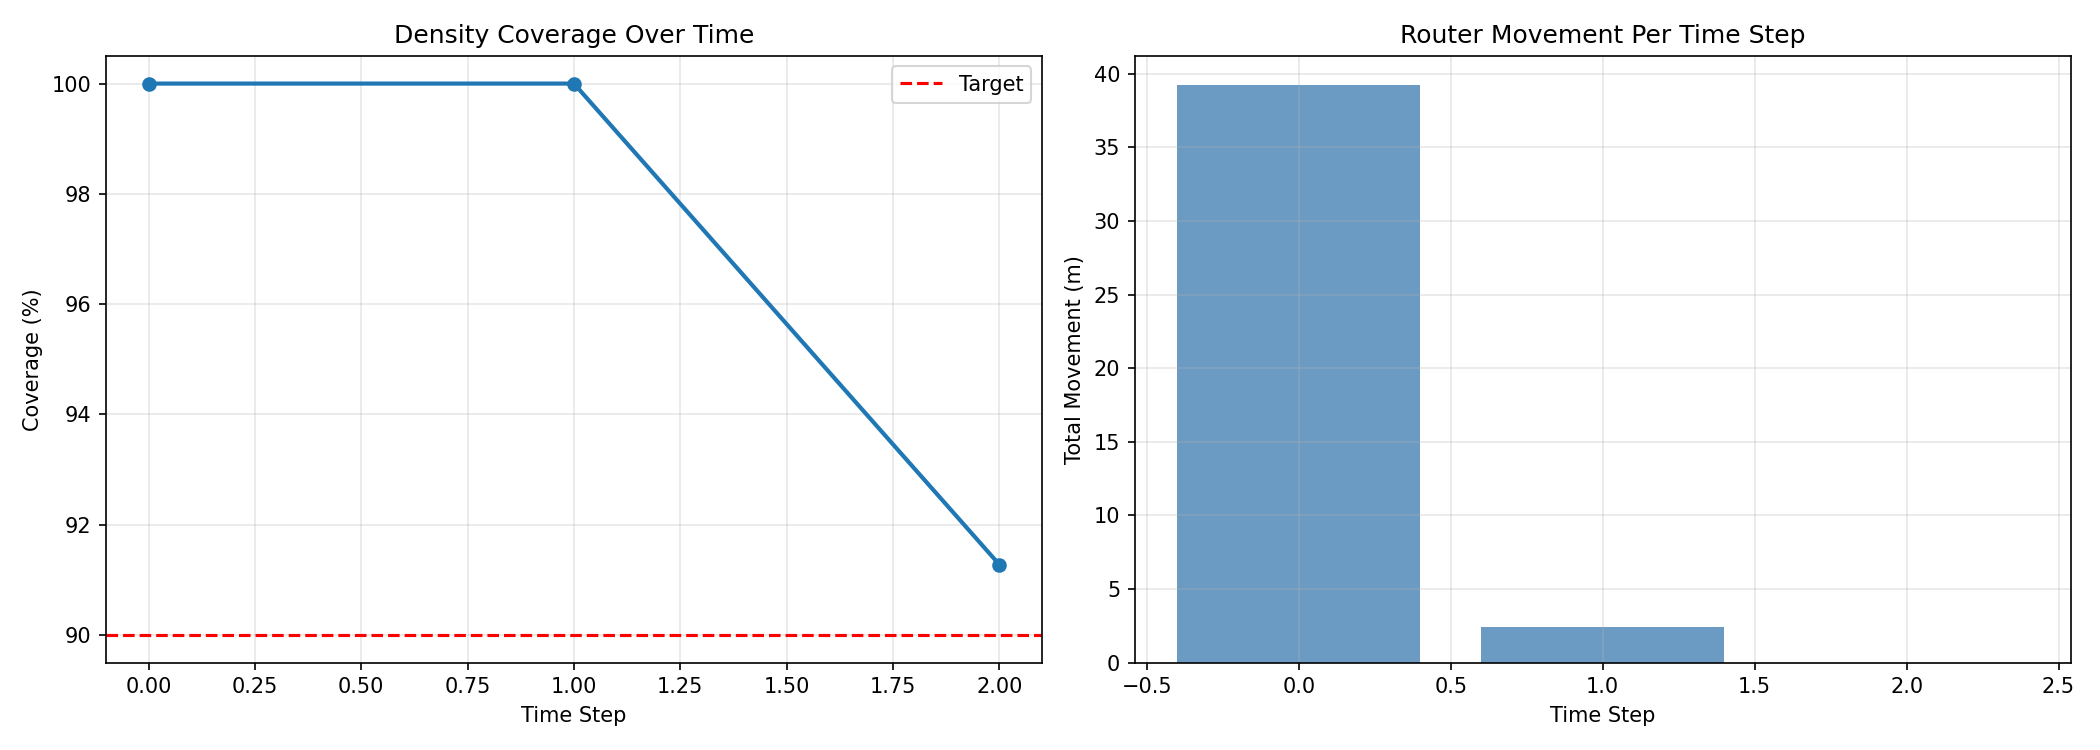
\includegraphics[width=0.85\textwidth]{coverage_over_time.png}
    \caption{Left: Density-weighted coverage percentage across time steps, with the 90\% target shown as a dashed red line. Right: Total router displacement (metres) per time step, showing sharply decreasing movement as the system stabilizes.}
    \label{fig:coverage}
\end{figure}


\subsection{4.4 Summary of Key Metrics}
\begin{itemize}
    \item \textbf{Coverage Improvement}: Static placement achieves only 16.6\% coverage; after APSO optimization, coverage reaches a perfect 100.0\% for initial steps and remains $\geq$91.3\% across dynamic crowd scenarios.
    \item \textbf{Dead Zone Reduction}: Up to 100\% elimination of poor-SINR areas (SINR\,$<$\,5\,dB), transforming the floor plan from predominantly unusable to near-uniform connectivity.
    \item \textbf{Optimization Speed}: Worst-case cold start $\sim$138\,s; warm-started incremental updates converge rapidly between 18\,s and 35\,s---well within the timescale of crowd dynamics.
    \item \textbf{Movement Efficiency}: Decreasing total displacement ($\sim$39\,m $\to$ $\sim$2.5\,m $\to$ $\sim$0\,m) across successive time steps confirms the system avoids redundant physical reconfiguration.
\end{itemize}

\section{5. Conclusion}
\begin{itemize}
    \item The concept is \textbf{validated through full-physics simulation} with both quantitative metrics and visual SINR heatmap evidence demonstrating coverage jumping from 16.6\% to 100.0\%.
    \item The coverage target of $\geq$90\% is \textbf{consistently achieved} across all three dynamic crowd scenarios (100.0\%, 100.0\%, 91.3\%), proving robustness to user mobility.
    \item Optimization is \textbf{real-time feasible}: even cold-start convergence completes in $\sim$2.3 minutes, with incremental updates taking between 18 and 35 seconds.
    \item The 4-tier escalation hierarchy is \textbf{validated}: total mechanical displacement drastically decreases in subsequent steps, reserving costly physical movement for significant reconfigurations only.
    \item The solution is \textbf{technically feasible}---motorized ceiling rail systems, THz transceiver hardware operating above 100\,GHz, and APSO are all commercially available or demonstrated technologies.
\end{itemize}

\end{document}
